\documentclass{beamer}

% Pacotes básicos 
\usepackage[utf8]{inputenc}
\usepackage{booktabs}
\usepackage{caption}
\usepackage{subcaption}
\usepackage{graphicx}
\usepackage{xcolor}
\definecolor{darkgreen}{rgb}{0.0, 0.5, 0.0}
\usepackage{amsmath}
\usepackage{amsfonts}
\usepackage{amssymb}
\usepackage{epstopdf}
\usepackage{physics}
\usepackage{csquotes}
\usepackage{url}
\usepackage[natbib=true,style=authoryear, backend=biber, useprefix=true]{biblatex}
\addbibresource{bibliografia.bib}

\usepackage{hyperref}
\hypersetup{
    colorlinks=false,
    linkcolor=blue,
    filecolor=magenta,      
    urlcolor=cyan,
    pdftitle={Overleaf Example},
    pdfpagemode=FullScreen,
    }

% \setbeamertemplate{footline}[frame number]
% \addtobeamertemplate{navigation symbols}{}{%
%     \usebeamerfont{footline}%
%     \usebeamercolor[fg]{footline}%
%     \hspace{1em}%
%     \insertframenumber/\inserttotalframenumber
% }



% Theme
\usetheme{Madrid} % Choose your preferred theme here
\useoutertheme[subsection=false]{miniframes}

\setlength{\fboxsep}{2pt}

\newcommand{\myconference}{CEWQO 2023}

\setbeamertemplate{footline}
{
  \leavevmode%
  \hbox{%
  \begin{beamercolorbox}[wd=.6\paperwidth,ht=2.25ex,dp=1ex,center]{author in head/foot}%
    \usebeamerfont{author in head/foot}\insertshortauthor
  \end{beamercolorbox}%
  \begin{beamercolorbox}[wd=.2\paperwidth,ht=2.25ex,dp=1ex,center]{title in head/foot}%
    \usebeamerfont{title in head/foot}\myconference
  \end{beamercolorbox}%
  \begin{beamercolorbox}[wd=.2\paperwidth,ht=2.25ex,dp=1ex,right]{date in head/foot}%
    \usebeamerfont{date in head/foot}\insertframenumber{} / \inserttotalframenumber\hspace*{2ex} 
  \end{beamercolorbox}}%
  \vskip0pt%
}
\setbeamertemplate{navigation symbols}{}






% Title Page
\title{Shadow tomography on general measurement frames}
\author{Luca Innocenti}
% \logo{
\includegraphics[scale=.03]{eqai-2023-logo.jpg}}
\date{CEWQO 2023}

% Content
\begin{document}


\section{Intro}

\begin{frame}
  \titlepage
  \begin{center}
      \scriptsize
  Ivan Palmisano, Salvatore Lorenzo, Francesco Albarelli, Alessandro Ferraro, Mauro Paternostro, Massimo Palma.
  \end{center}
  \hfill
\includegraphics[height=1cm]{figures/logo-unipa-2020.png}
\includegraphics[height=1.cm]{figures/qub_logo.png}\quad
\includegraphics[height=1.cm]{figures/unimilogo.png}
\end{frame}


\begin{frame}
  \frametitle{The roadmap...}
  % \framesubtitle{What is a reservoir computer?}
  
  \begin{itemize}\setlength\itemsep{1em}
      \item Present a conceptually simple strategy to estimate properties of input states in a general scenario.
      \item Demonstrate the tight connections between the frameworks of linear state tomography and shadow tomography.
      \item Characterise the class of measurements that allows estimating target properties with favourable scalings with respect to state dimension.
  \end{itemize}
  \vspace{1cm}
  \begin{flushright}\scriptsize
      \textit{Shadow tomography on general measurement frames}, \href{https://arxiv.org/abs/2301.13229}{arXiv:2301.13229},
      \\
      \textit{Potential and limitations of quantum extreme learning machines}, \href{https://arxiv.org/abs/2210.00780}{arXiv:2210.00780}
  \end{flushright}  
\end{frame}

\begin{frame}{\hspace{9.5cm}... the end}
    \begin{itemize}
    \setlength\itemsep{1em}
        \item \colorbox{red!10}{\parbox[t]{\dimexpr\linewidth-2\fboxsep}{The standard formulation of shadow tomography \textit{(projective measurements after random unitaries plus post-processing)} allows efficient estimation of many properties of input states.}}
        \item \colorbox{green!10}{\parbox[t]{\dimexpr\linewidth-2\fboxsep}{%
            We can simultaneously \textit{generalise} and \textit{simplify} the standard approach, maintaining and explaining the performance guarantees.
        }}
        \item \colorbox{orange!10}{\parbox[t]{\dimexpr\linewidth-2\fboxsep}{%
            We gain a completely general estimation procedure with attached well-characterised performance guarantees.
        }}
    \end{itemize}
\end{frame}


\section{Shadow tomography}

\begin{frame}{What's \textit{shadow tomography}?}
% \setbeamercovered{transparent=30}

    \begin{itemize}\small\setlength\itemsep{1em}
        \item \colorbox{orange!20}{\parbox[t]{\dimexpr\linewidth-2\fboxsep}{%
        Can we estimate properties of a $D$-dimensional state $\rho$ with a number of measurements that \textit{does not} scale with $D$?}}
        \item {\color{green!45!black} The shadow tomography protocol allows to estimate $\trace(\mathcal O_1\rho),...,\trace(\mathcal O_M\rho)$ within additive error $\epsilon$ performing $N\sim \log(M) \max_i \|\mathcal O_i\|_{\rm sh}^2/\epsilon^2$.}
    \end{itemize}

    \begin{center}
    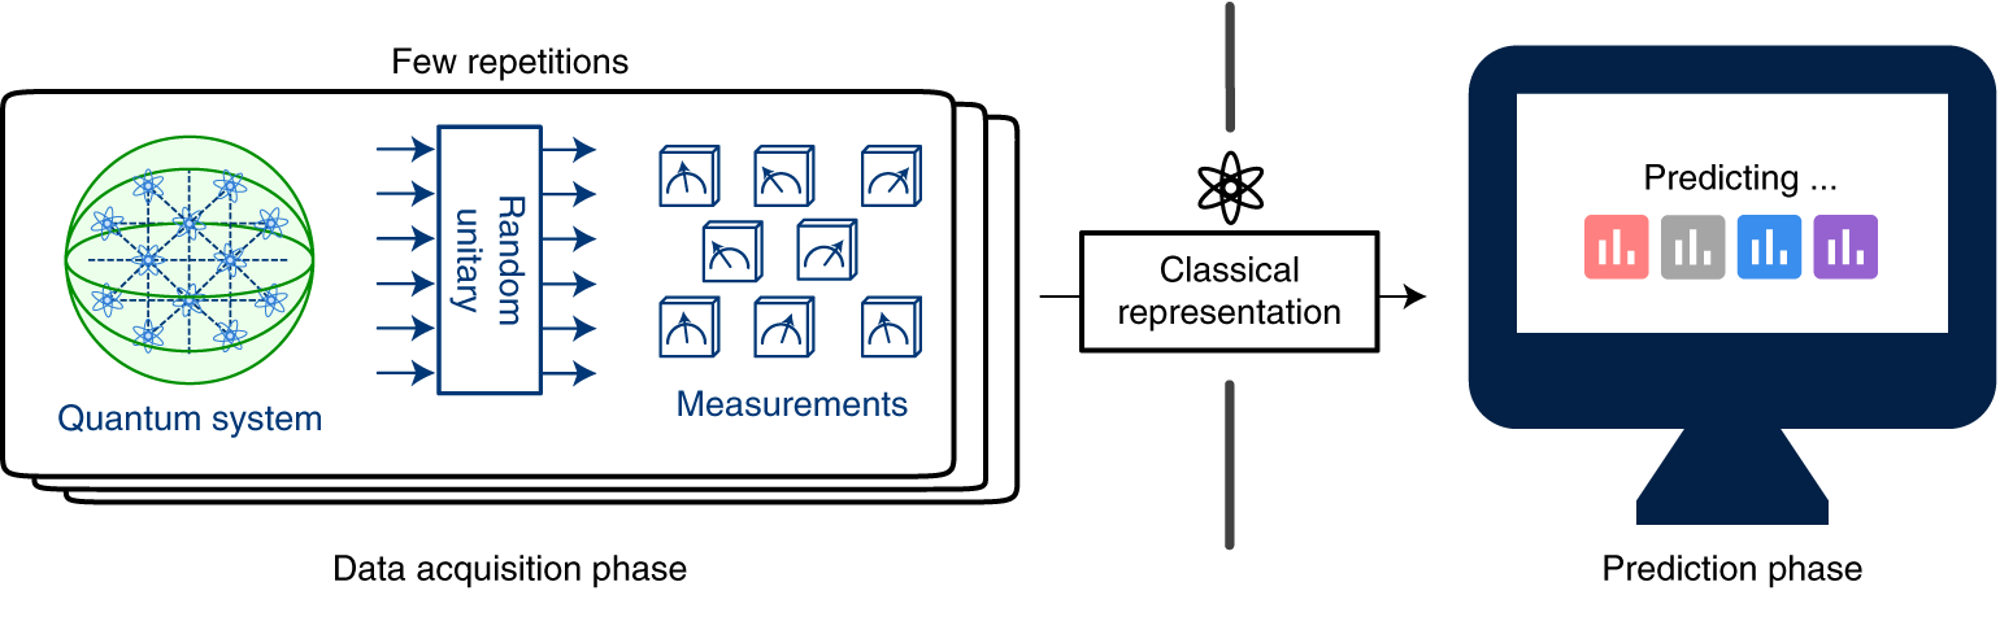
\includegraphics[width=0.7\textwidth]{figures/shadowtomographyscheme_concise.png}
    \end{center}
    \vspace{1cm}
    \begin{itemize}\scriptsize
        \item Aaronson, \textit{Shadow Tomography of Quantum States} \href{https://arxiv.org/abs/1711.01053}{arXiv:1711.01053}.
        \item
        Brandão et al, \textit{Quantum SDP Solvers}
        \href{https://arxiv.org/abs/1710.02581}{arXiv:1710.02581}.
        \item Huang et al. ``\textit{Predicting many properties of a quantum system from very few measurements.}'' \href{https://arxiv.org/abs/2002.08953}{arXiv:2002.08953}
    \end{itemize}
    

\end{frame}



\begin{frame}
\frametitle{Classical shadows --- how do they work?}

\setbeamercovered{transparent=30} % Make the text that has not yet appeared be 50% transparent


    \begin{enumerate}\small\setlength\itemsep{0.8em}
        \item Evolve $\rho$ with a random unitary $U$: $\rho\mapsto U\rho U^\dagger$.\pause
        \item Perform a projective measurement $\{\ketbra b\}_b$, obtaining an outcome $\hat b\in\{0,1\}^n$ (with probability $\langle b|U\rho U^\dagger|b\rangle$).\pause
        \item Compute (in post-processing) the ``classical shadows''
        \begin{equation*}
            \hat\rho = \mathcal M^{-1}(U^\dagger\ketbra*{\hat b} U),
            \qquad
            \mathcal M(\rho) \equiv \mathbb{E}[U^\dagger\ketbra*{\hat b} U].
        \end{equation*}\pause
        \item Repeat $N$ times, obtaining $N$ shadows $\hat\rho_i$. These give the state on average: $\mathbb E[\hat \rho]=\rho$.
        To estimate $\mathcal O$, use $\hat o_i=\trace(\mathcal O\hat\rho_i)$, and then compute the sample mean:
        \begin{equation*}
            \overline o_N \equiv\frac{1}{N} \sum_{i=1}^N \hat o_i
            = \frac{1}{N} \sum_{i=1}^N \trace(\mathcal O\mathcal M^{-1}(U^\dagger \ketbra*{\hat b_i} U) ).
        \end{equation*}
    \end{enumerate}
\end{frame}

\begin{frame}{What's $\mathcal M$?}
\setbeamercovered{transparent=30}
    \begin{center}
    \begin{beamerboxesrounded}[shadow=true]{Huang et al. shadow scheme}
    \textit{
    Measure $U\rho U^\dagger$; 
    obtain $b$; 
    compute $\hat\rho=\mathcal M^{-1}(\ketbra*{b})$; 
    compute $\trace(\mathcal O\hat\rho)$.
    }
    \end{beamerboxesrounded}
    \end{center}
    \begin{itemize}\small
        \item The map $\mathcal M$ is the channel defined as $\mathcal M(\rho)=\mathbb{E}[U^\dagger \ketbra*{\hat b}U]$, \textit{i.e.}
        \begin{equation*}
        \mathcal M(X) \equiv \int dU\,
        \sum_b
        \textcolor{blue}{\langle b|U\rho U^\dagger|b\rangle}
        \,\, \textcolor{orange}{U^\dagger\ketbra*{b} U}.
        \end{equation*} \pause
        \item $\mathcal M$ is known beforehand, and can be computed explicitly. It is (typically) a depolarising channel, which makes computing $\mathcal M^{-1}$ easy.\pause
        \item \colorbox{yellow!15}{\parbox[t]{\dimexpr\linewidth-2\fboxsep}{$\mathcal M$ is \textit{not} an actual dynamic that needs to be implemented. Nor $\mathcal M^{-1}$ is generally a channel. They are only used in post-processing.}}
    \end{itemize}
\end{frame}


\begin{frame}{Toy example of single-qubit shadow tomography}
    \begin{center}
    \begin{beamerboxesrounded}[shadow=true]{Huang et al. shadow scheme}
    \textit{
    Measure $U\rho U^\dagger$; 
    obtain $b$; 
    compute $\hat\rho=\mathcal M^{-1}(\ketbra*{b})$; 
    compute $\trace(\mathcal O\hat\rho)$.
    }
    \end{beamerboxesrounded}
    \end{center}
    \begin{itemize}\small
        \item Consider \textit{e.g.} measuring a single qubit $\rho$ with uniformly random unitaries $U\in\mathbf U(2)$, and computational basis measurements $\{\ketbra0,\ketbra1\}$. Then
        \begin{equation*}
            \mathcal M(X)
            % = \int_{\mathbf{U}(1)} dU\,
            % \sum_{b=0,1} \langle b|U\rho U^\dagger|b\rangle \,\, U^\dagger \ketbra*{b} U
            = \frac13 X + \frac23 \trace(X)\frac{I}{2},
            \qquad
            \mathcal M^{-1}(Y) = 3 Y - I.
        \end{equation*}
        \item \textbf{Procedure}:
        \colorbox{yellow!10}{(1)}
        Pick $U_1\in\mathbf U(1)$. Measure $U_1\rho U_1^\dagger$. Get $b=0$. Store
        $\hat\rho_1 = 3 U_1^\dagger\ketbra*{0} U_1 - I$. %
        \colorbox{green!10}{(2)}
        Take another $\rho$ and $U_2\in\mathbf U(2)$. Measure $U_2\rho U_2^\dagger$. Get $b=1$. Store $\hat\rho_2=3U_2^\dagger\ketbra*{1} U_2-I$.
        \colorbox{red!10}{($...n$)} Take the average.
    \end{itemize}
\end{frame}


\begin{frame}{Performance guarantees with random unitaries}\small
    \begin{center}
    \begin{beamerboxesrounded}[shadow=true]{Huang et al. shadow scheme}
    \textit{
    Measure $U\rho U^\dagger$; 
    obtain $b$; 
    compute $\hat\rho=\mathcal M^{-1}(\ketbra*{b})$; 
    compute $\trace(\mathcal O\hat\rho)$.
    }
    \end{beamerboxesrounded}
    \end{center}
    \begin{itemize}\small
        \item We get estimates $\hat o_1,..,\hat o_M$ for observables $\mathcal O_1,..., \mathcal O_M$ such that
        \begin{equation*}
            \operatorname{Prob}(
            |\hat o_i - \trace(\mathcal O_i\rho)|\le\epsilon,\,\,\forall i=1,...,M) \ge1-\delta,
        \end{equation*}
        with a number of measurements
        \begin{equation*}
            N \ge C \frac{2\log(2M/\delta)}{\epsilon^2}
            \max_{1\le i \le M} \left\|\mathcal O_i - \trace(\mathcal O_i) I / d\right\|_{\rm sh},
        \end{equation*}
        where
        \begin{equation*}
            \|\mathcal O\|_{\rm sh}^2 = \max_\sigma
            \int dU\sum_b
            \langle b|U \sigma U^\dagger|b\rangle
            \langle b| U\mathcal M^{-1}(\mathcal O)U^\dagger |b\rangle.
        \end{equation*}
        \item In a number of cases of interest, $\|\mathcal O\|_{\rm sh}^2 \le 3\trace(\mathcal O^2) \simeq O(1)$.
    \end{itemize}
\end{frame}

\section{Cool... but \textit{why} does this work?}

\begin{frame}{Is there a more natural \textit{framing}?}
    \begin{itemize}\setlength\itemsep{1em}
        \item We want to show that this formalism is actually extremely natural and conceptually simple.
        \item In the process, show that this scheme can be generalised, and works with \textit{arbitrary} POVMs.
        \item Dimension-independent scalings \textit{do not} apply in all cases, but we can characterise entire classes of POVMs where they do.
    \end{itemize}
\end{frame}

\begin{frame}{And now for something completely different... frames!}
    \begin{itemize}\setlength\itemsep{0.5em}
        \item \textit{Frame}work to deal with overcomplete ``bases''. A ``frame'' is a set of vectors $\{\mathbf v_k\}\subset V$ that span $V$.
        \item Given a frame, there's always a --- \textit{not necessarily unique} --- \textit{dual frame}: a set of vectors $\{\tilde{\mathbf v}_k\}$ such that any $\mathbf x\in V$ decomposes as
        \begin{equation*}
            \mathbf x = \sum_k \langle \tilde{\mathbf v}_k, \mathbf x\rangle \mathbf v_k
            = \sum_k \langle \mathbf v_k, \mathbf x\rangle \tilde{\mathbf v}_k.
        \end{equation*}
        \item A canonical way to find a dual frame is to define the \textit{frame operator}
        \begin{equation*}
            S \equiv \sum_k \mathbf v_k \mathbf v_k^\dagger,
        \end{equation*}
        and then build the dual frame as $\tilde{\mathbf v}_k = S^{-1}(\mathbf v_k)$.
    \end{itemize}
\end{frame}

\begin{frame}{Frame theory - toy example}
    \begin{itemize}
        \item In $\mathbb{R}^2$, the set $\{\mathbf v_i\}_{i=1}^3=\{(1,0), (0,1), (1,1)\}$ is a frame. The frame operator is
        \begin{equation*}
            S = \begin{pmatrix}
                2 & 1 \\ 1 & 2.
            \end{pmatrix},
            \qquad
            S^{-1} = \frac13\begin{pmatrix}
                 2 & -1 \\ -1 & 2
            \end{pmatrix}.
        \end{equation*}
        The canonical dual frame is
        \begin{equation*}
            \tilde{\mathbf v}_1 = \frac13(2,-1),
            \qquad
            \tilde{\mathbf v}_2 = \frac13(-1,2),
            \qquad
            \tilde{\mathbf v}_2 = \frac13(1,1).
        \end{equation*}
        \item Any $\mathbf x\equiv (x_0,x_1)$ can be decomposed as
        \begin{equation*}
            \mathbf x = \frac13(2x_0-x_1) \binom{1}{0}
            +
            \frac13(-x_0+2x_1) \binom{0}{1} +
            \frac13(x_0+x_1) \binom{1}{1}.
        \end{equation*}
    \end{itemize}
\end{frame}


\begin{frame}{\textit{Measurement} frames}
\setbeamercovered{transparent=30}
    \begin{itemize}
        \item Apply frame theory to decompose states via POVMs:
        given any \textit{informationally complete} POVM $\boldsymbol\mu\equiv\{\mu_b\}_b$, and \textit{any} \textcolor{darkgreen}{dual measurement frame} $\tilde{\boldsymbol \mu}\equiv\{\tilde{ \mu}_b\}_b$ we get the decomposition
        \begin{equation*}
            \rho = \sum_b
            \underbrace{\langle \mu_b,\rho\rangle}_{\equiv\trace(\mu_b\rho)}
            \tilde\mu_b.
        \end{equation*}\pause
        \item A canonical choice of dual frame is $\tilde\mu_b = S^{-1}(\mu_b)$, where
        \begin{equation*}
            S = \sum_b |\mu_b\rangle\!\rangle\!\langle\!\langle \mu_b|,
            \qquad
            S(X) \equiv \sum_b \trace(\mu_b X)\mu_b.
        \end{equation*}\pause
        \item \colorbox{yellow!30}{This choice is not unique, nor \textit{optimal}}.
    \end{itemize}
\end{frame}

\begin{frame}{Estimation theory and measurement frames}
    \begin{itemize}
        \item Dual measurement frames correspond to \textit{unbiased state estimators}. Given any dual frame $\{\tilde\mu_b\}$, the function $\hat f(b)\equiv\tilde\mu_b$ is an unbiased estimator for \textit{any} $\rho$, meaning
        \begin{equation*}
            \mathbb{E}[\hat f|\rho]
            \equiv \sum_b \underbrace{\langle\mu_b,\rho\rangle}_{p_b(\rho)} \hat f(b)
            =\rho, \,\,\forall \rho.
        \end{equation*}
        \item {{\bfseries\itshape Dual bases $\simeq$ unbiased state estimators}}: there's a bijection between dual measurement frames $\{\tilde\mu_b\}$ and unbiased estimators $\hat f$.
        \item \textbf{Observable estimators} --- Building estimators as
        \begin{equation*}
            \hat o(b) \equiv \langle \mathcal O,\hat f(b)\rangle =
            \langle \mathcal O,\tilde\mu_b\rangle
        \end{equation*}
        we have
        % \begin{equation*}
            $\mathbb{E}[\hat o|\rho] = \langle\mathcal O,\rho\rangle.$
        % \end{equation*}
        % \item \textbf{What's the ``best'' such unbiased estimator?}
        % A standard way to answer this question is to look for $\hat f$ minimising the variance:
        % \begin{equation*}
        %     \operatorname{Var}[\hat f|\rho] =
        %     \sum_b \langle \mu_b,\rho\rangle \hat f(b)^2
        %     - \rho^2
        % \end{equation*}
    \end{itemize}
\end{frame}

\section{Shadow tomography via frames}

\begin{frame}{Back to \textcolor{black}{\textbf{shadows}}: a general estimation strategy}
\setbeamercovered{transparent=30}
    \begin{itemize}\setlength\itemsep{1em}
        \item We thus get the general estimation recipe for any given $\boldsymbol\mu$: pick a dual measurement frame $\tilde{\boldsymbol\mu}$; get your complimentary unbiased estimator $\hat f$; enjoy estimating. \pause
        \item \colorbox{orange!15}{\parbox[t]{\dimexpr\linewidth-2\fboxsep}{Shadow tomography amounts to building unbiased estimators via measurement frames, \textit{for specific choices of POVM $\boldsymbol\mu$.}}} \pause
        \item In this sense, \colorbox{yellow!20}{\textbf{shadow tomography} $\simeq$ \textcolor{darkgreen}{\textbf{linear state tomography}}} (though \textit{shadow tomography} isn't about doing tomography at all). \pause
        \item Whether dimension-independent estimation is possible depends exclusively on the properties of $\boldsymbol\mu$.
    \end{itemize}
\end{frame}


\begin{frame}{Variances vs estimation errors}\small
    \begin{itemize}
        \item To determine the number of measurement outcomes required to achieve a given accuracy, the first thing to look at is the \textbf{estimator variance}:
        \begin{equation*}
            \operatorname{Var}[\hat o|\rho] =
            \sum_b \langle\mu_b,\rho\rangle \hat o(b)^2
            - \langle \mathcal O, \rho\rangle^2,
            \qquad \hat o(b)\equiv \langle \mathcal O,\tilde\mu_b\rangle.
        \end{equation*}
    \end{itemize}
        % \item
    \begin{center}
    \begin{beamerboxesrounded}[shadow=true]{Why care about the variance?}
    \textcolor{darkgreen}{
    From standard statistical considerations, bounds on the variance translate on bounds on the statistics required to achieve target accuracies. \textit{E.g.}
        \begin{equation*}
            \text{Pr}(|\overline X_N-\mu|\ge \epsilon) \le \frac{\operatorname{Var}(X)}{N\epsilon^2},
        \end{equation*}
    which means $\operatorname{Pr}(|\overline X_N-\mu|\ge\epsilon)\le\delta$ if $N\ge \operatorname{Var}(X)/\delta\epsilon^2$.
    }
    \end{beamerboxesrounded}
    \end{center}
\end{frame}


\begin{frame}{So... \textit{when} does $\boldsymbol\mu$ allow ``efficient estimation''?}
\setbeamercovered{transparent=30}
    \begin{itemize}
        \item Within this framework, we can explicitly work the ``optimal'' choice of dual frame/unbiased estimator for any given $\boldsymbol\mu$. Namely:
        \begin{equation*}
            \tilde\mu_b^{\rm can} \equiv \frac{ S^{-1}_{\rm can}(\mu_b)}{\trace(\mu_b)/d},
            \qquad
            S_{\rm can} \equiv \sum_b \frac{|\mu_b\rangle\!\rangle\!\langle\!\langle\mu_b|}{\trace(\mu_b)/d}
        \end{equation*}
        gives minimum (on average) variance.
        \pause
        \item You can also work out the estimator with minimum variance when the state is some specific $\rho$:
        \begin{equation*}
            \tilde\mu_b^{(\rho)} = \frac{S^{-1}_\rho(\mu_b)}{\langle\mu_b,\rho\rangle},
            \qquad
            S_\rho \equiv \sum_b \frac{|\mu_b\rangle\!\rangle\!\langle\!\langle\mu_b|}{\langle \mu_b,\rho \rangle }.
        \end{equation*}
        \item \colorbox{yellow!20}{In fact, $S_\rho$ is precisely the relevant Fisher information matrix.}
    \end{itemize}
\end{frame}

\begin{frame}{How to \textit{design} the ``best'' $\boldsymbol\mu$?}
    \begin{itemize}
        \item \textbf{For any rank-1 POVM that gives a weighted 2-design}, 
        \begin{equation*}
            \mu_b = w_b \ketbra{\psi_b},
            \qquad
            \sum_b w_b \ketbra{\psi_b}^{\otimes 2}
            = \frac{\Pi_{\rm sym} }{\binom{d+1}{2}},
        \end{equation*}
        frame superoperator and canonical estimators are particularly simple, and the \textbf{average variance is}
        \begin{equation*}
            \overline{\operatorname{Var}[\hat o]} =
            Vd \left(\frac{d^2+d-2}{d^2-1}\right),
            \quad
            V \equiv \langle\mathcal O^2\rangle_{I/d}
            -\langle \mathcal O\rangle_{I/d}^2.
        \end{equation*}
        \item For \textbf{3}-designs: we also get closed formulas for non-averaged variances:
        \begin{equation*}
            \operatorname{Var}[\hat o|\rho,\mathcal O]
            \sim \trace(\mathcal O^2) + 2\trace(\mathcal O^2\rho)
            - \trace(\mathcal O\rho)^2
            \le 3 \trace(\mathcal O^2),
            \qquad d\gg1.
        \end{equation*}
    \end{itemize}
\end{frame}


\begin{frame}{Connection with Huang et al. approach}
\setbeamercovered{transparent=30}
    \begin{center}
    \begin{beamerboxesrounded}[shadow=true]{Huang et al. shadow scheme}
    \textit{
    Measure $U\rho U^\dagger$; 
    obtain $b$; 
    compute $\hat\rho=\mathcal M^{-1}(\ketbra*{b})$; 
    compute $\trace(\mathcal O\hat\rho)$.
    }
    \end{beamerboxesrounded}
    \end{center}
    \begin{itemize}\setlength\itemsep{0.5em}
        \item \colorbox{orange!15}{\parbox[t]{\dimexpr\linewidth-2\fboxsep}{
            Applying this tech to \textit{covariant measurements}, \textit{i.e.}
            $\mu_{U,b} = U^\dagger \ketbra{b} U$, we 
            % \begin{equation}
            % \end{equation}
            get precisely the ``standard'' shadow tomography scheme.
        }} \pause
        \item The channel $\mathcal M$ is the \textit{frame (super)operator} corresponding to $\{\mu_{U,b}\}$, and $\mathcal M^{-1}(\ketbra{b})$ are the \textit{dual frame elements}. \pause
        \item The ``shadow norm'' $\|\mathcal O\|_{\rm sh}$ is just the maximised variance. \pause
        \item The general performance guarantees are due to \textit{random unitary measurements} forming a 3-design (or more).
    \end{itemize}
\end{frame}

\begin{frame}{Example: random unitaries vs MUBs}
\setbeamercovered{transparent=30}
    \begin{center}
    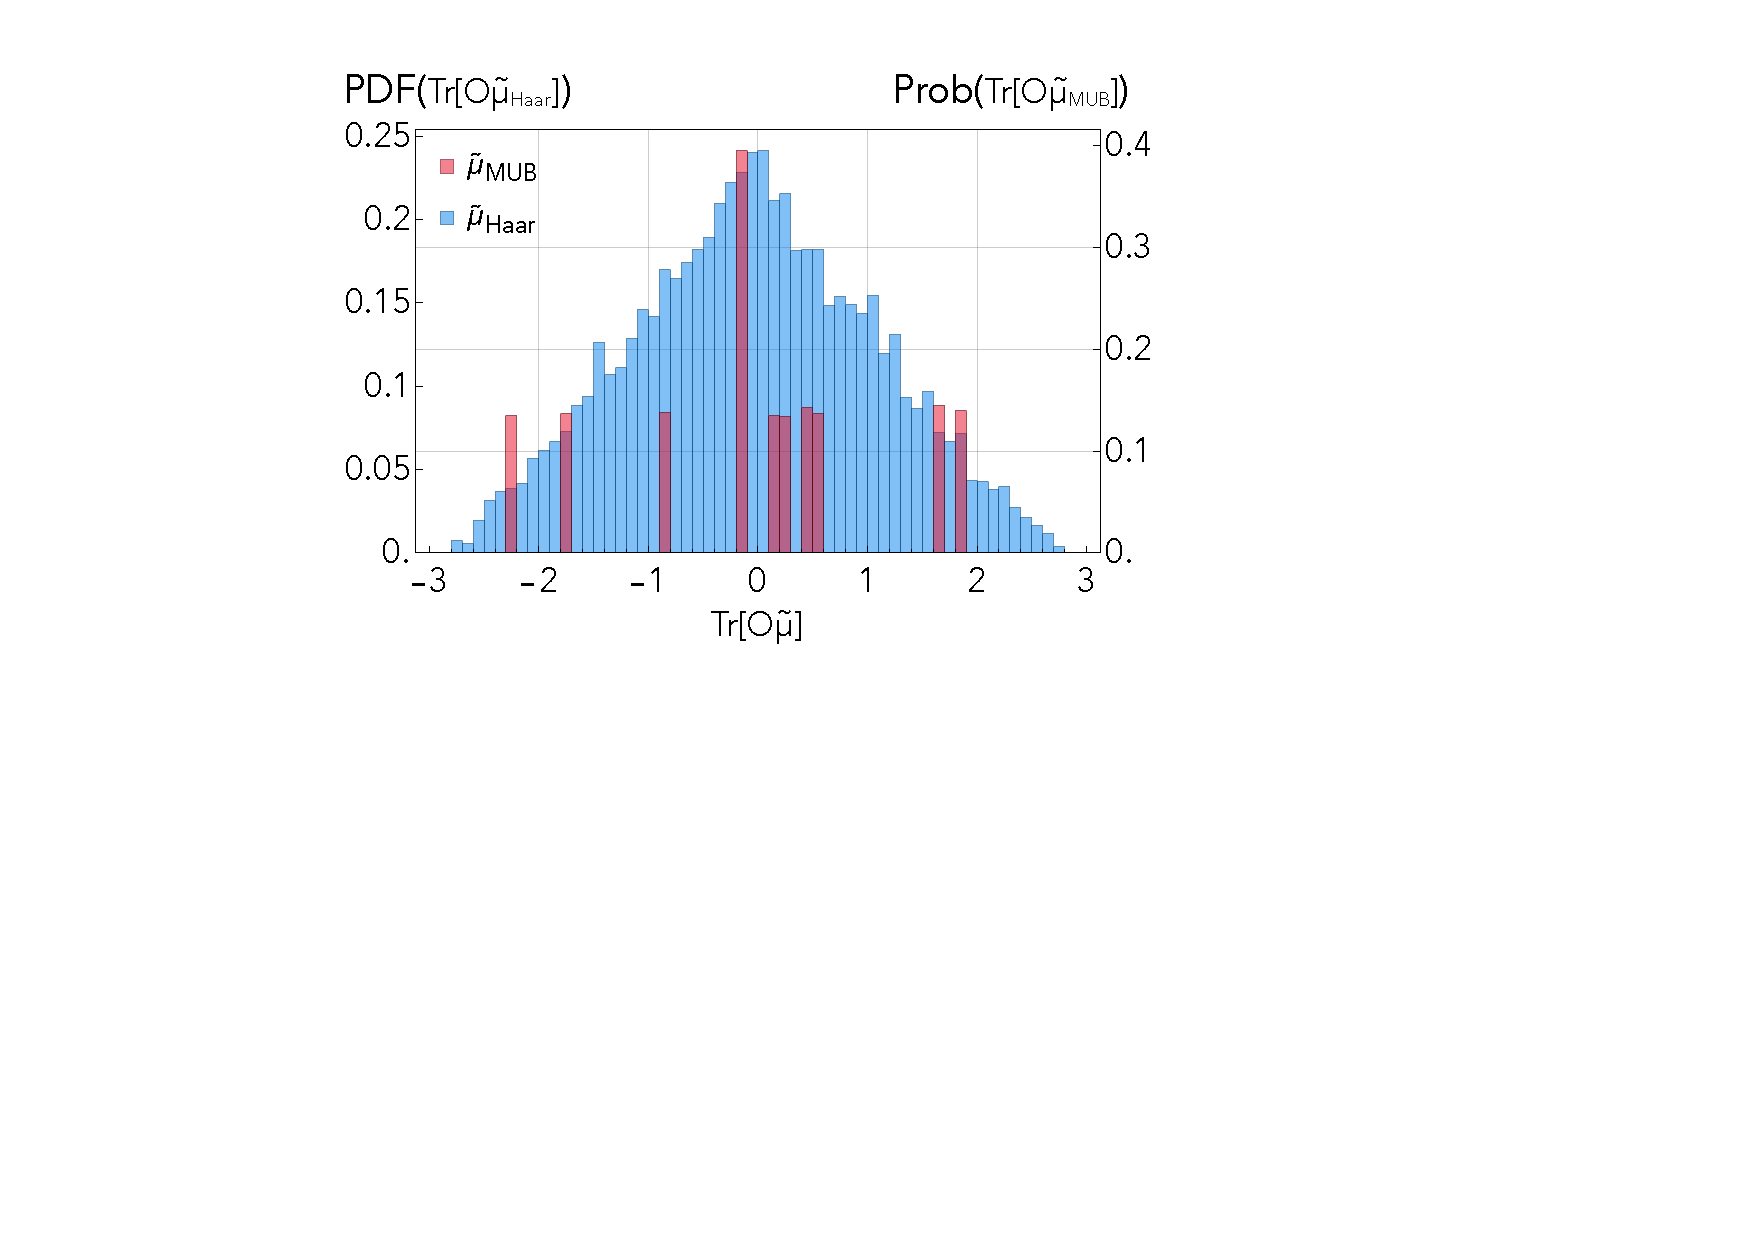
\includegraphics[width=0.7\textwidth]{figures/hist_MUB_Preskill.pdf}
    \end{center}
\end{frame}

% \begin{frame}
% \frametitle{Training QELMs vs measurement reconstruction}

% \begin{itemize}
%     \item We can show that the process of training a QELM is equivalent to a form of (limited) measurement tomography:
%     the training problem
%     \begin{equation}
%         \sum_b w_b\operatorname{tr}(\mu_b\rho_i^{\rm tr}) = \operatorname{tr}(\mathcal O\rho_i^{\rm tr}), \quad\forall i,
%     \end{equation}
%     has solution
%     \begin{equation}
%         \mathbf w = \operatorname{tr}(\mathcal O \boldsymbol\mu^\star).
%     \end{equation}
%     In words, the training produces a representation of the \textit{dual} of the effective measurement, projected on the target observables.
% \end{itemize}
    
% \end{frame}


% \begin{frame}
% \frametitle{QELM, error estimates}
%     \begin{itemize}
%         \item Using these estimators we can work out the associated variances, and thus estimate the statistics necessary to recover information within a given accuracy:
%         \begin{equation}
%             \operatorname{Var}[\hat o] =
%             \sum_b\operatorname{tr}(\mu_b \rho) \operatorname{tr}(\mathcal O\hat\rho(b))^2 - \operatorname{tr}(\mu_b \rho)^2.
%         \end{equation}
%         \item When the effective measurement is sufficiently symmetric (gives a 2-design) the average variance has the optimal scaling:
%         \begin{equation}
%             \overline{\operatorname{Var}[\hat o]} =
%             Vd \left(\frac{d^2+d-2}{d^2-1}\right),
%             \quad
%             V\equiv \langle\mathcal O^2\rangle_{I/d}-\langle\mathcal O\rangle_{I/d}^2.
%         \end{equation}
%         \item $M$ observables can be estimated within additive error $\epsilon$ with probability $1-\delta$ with statistics $N\sim \frac{\log(M)}{\epsilon^2}\log(2/\delta)$.
%     \end{itemize}
% \end{frame}


\begin{frame}
  \frametitle{Conclusion}
  \begin{itemize}\setlength\itemsep{0.5em}
      \item We take the approach to shadow tomography via random unitaries, and ``understand it'' as the natural process of looking for unbiased state estimators for a given $\boldsymbol\mu$.
      \item We directly trace back the performance guarantees to symmetry properties (in the sense of $t$-designs) of POVMs.
      \item We gain a general recipe to figure out if and when a given measurement apparatus can be used to efficiently estimate stuff.
      \item In the context of \textit{quantum reservoir computing}, this allows a deeper insight into the kinds of reservoirs that allow estimation of target features; performing supervised learning training of a reservoir provides a specific dual measurement frame.
  \end{itemize}
\end{frame}


\begin{frame}{QELMs, single-shot regime}

\begin{itemize}
    \item Thinking of QELMs from a similar ``single-shot perspective'': look for the best estimators operating on individual measurement outcomes.
    \item Via a generalised shadow tomography \textit{frame}work, we find the optimal unbiased estimator to recover $\mathcal O$:
    \begin{equation}
        \hat o(b) = \operatorname{tr}(\mathcal O \hat\rho(b)),
        \quad
        \hat\rho(b)\equiv  \left(\sum_b \frac{|\mu_b\rangle\!\rangle\!\langle\!\langle \mu_b|}{\operatorname{tr}(\mu_b)} \right)^{-1}
        \frac{\mu_b}{\operatorname{tr}(\mu_b)}
    \end{equation}
    \item We show that the standard QELM training produces the estimator:
    \begin{equation}
        \hat o'(b) = \operatorname{tr}(\mathcal O\hat\rho'(b)),
        \quad \hat\rho'(b) \equiv
        \left(\sum_b|\mu_b\rangle\!\rangle\!\langle\!\langle\mu_b|\right)^{-1}\mu_b
    \end{equation}
\end{itemize}
\end{frame}


\end{document}
